\section{Copyright Clean Collection Process}
We believe that the continued development and use of AI systems should be predicated on such systems being both legally and ethically compliant, both in the current environment and in the wake of future regulatory and legislative changes.  In this section, we introduce the Kelvin Legal Large Language Model (KL3M) dataset, the largest dataset developed to date that respects the moral and legal rights of copyright holders. Our approach aims to circumvent the need for reliance on ``fair use" arguments by ensuring all data in the KL3M dataset is either in the public domain or explicitly licensed for unrestricted use.


\subsection{Copyright Filtration Process}
To build KL3M, we developed a multi-part filtration process designed to determine whether a given data source may be used without significant restriction. The test is based on a series of conditional assessments: if the data passes a test, we include it in the KL3M dataset; if the data does not pass the test, we move on to the next test. Data that does not pass any of our tests is not included in the KL3M dataset.  We describe the process below but also highlight the steps in Figure \ref{fig:CopyrightFlowchart} below.

\begin{figure}[ht!]
\centering
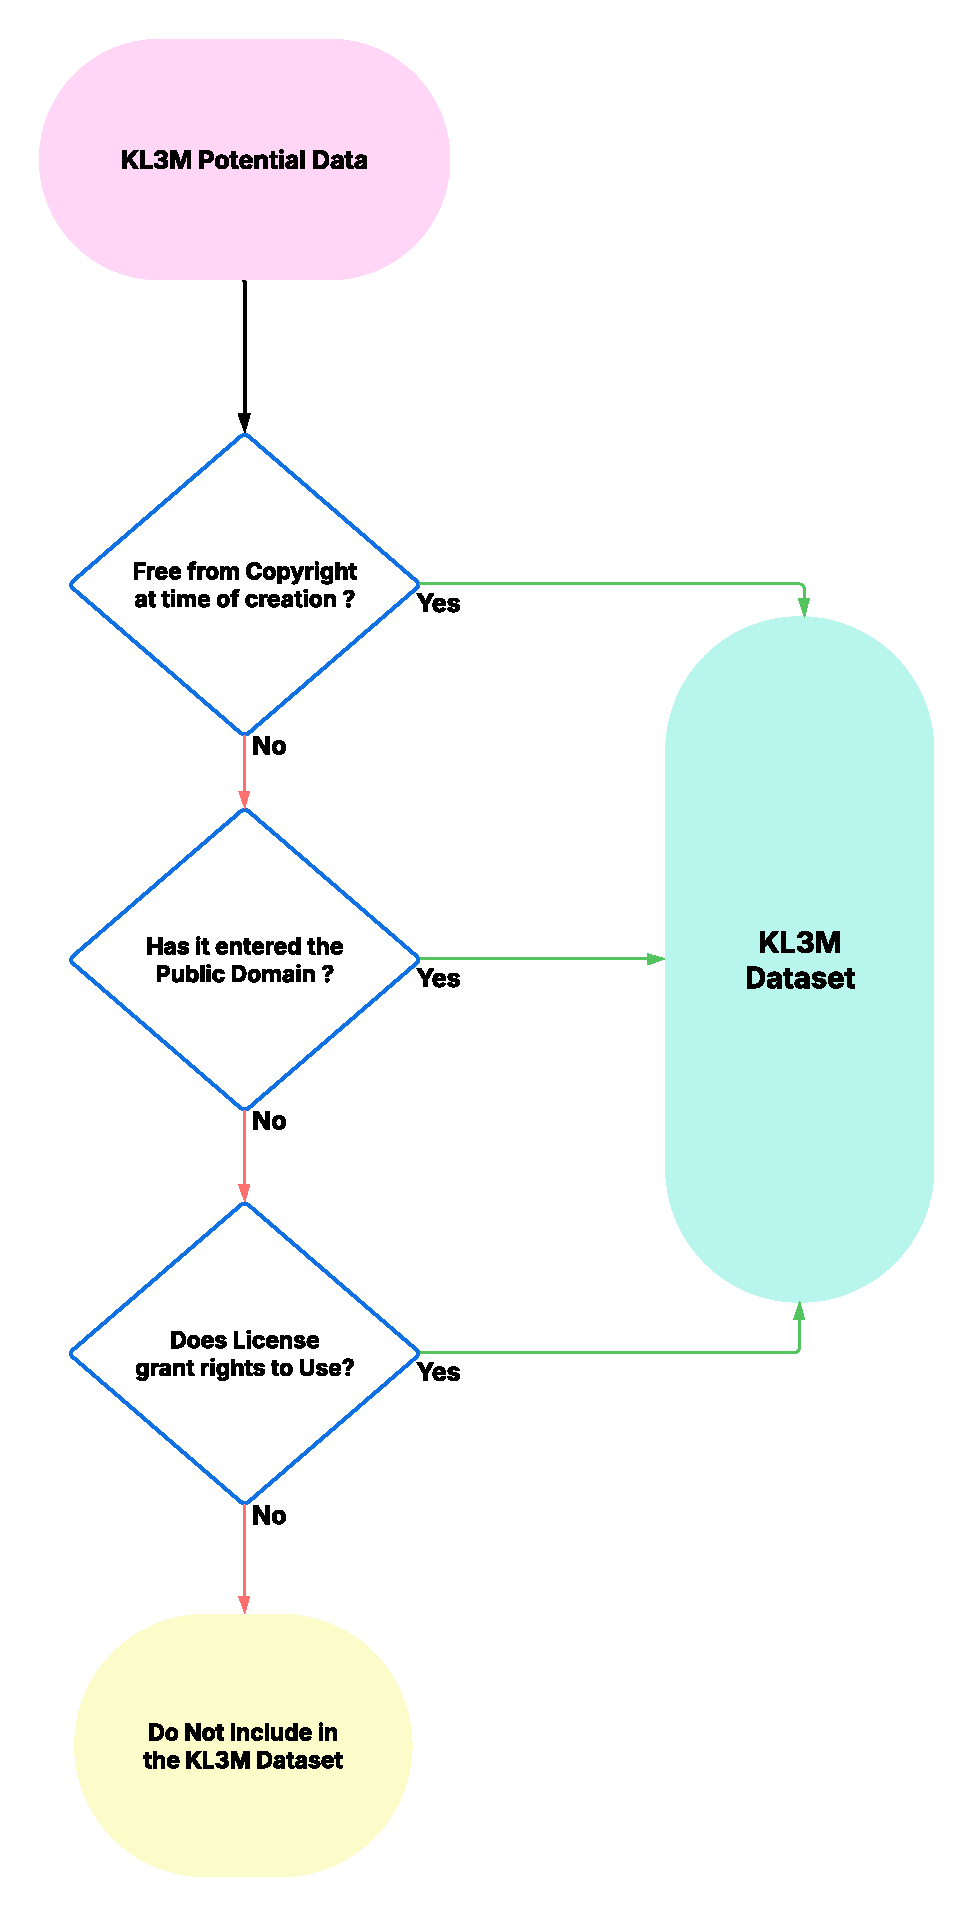
\includegraphics[width=70mm]{CopyrightFlowchart.pdf}
\caption{Overview of the Copyright Filtration Process}
\label{fig:CopyrightFlowchart}
\end{figure}

\subsubsection{Test 1 - Free from Copyright Protection}
Our first test is to determine whether the content is free from copyright \textbf{at the time of its creation}. A substantial percentage of content contained within the KL3M dataset meets this test and was thus eligible for inclusion.

Works of the United States government, for example, are not eligible for copyright protection under 17 U.S.C. § 105 (``Copyright protection under this title is not available for any work of the United States Government").  Specifically, work created by a federal government employee or officer is in the public domain, provided that the work was created in that person’s official capacity. 

A separate but related concept is the ``government edict doctrine."  This doctrine, developed through the common law, denies copyright protection to official ``government edicts."\footnote{The doctrine is long standing and dates back to \textit{Wheaton v. Peters}, 33 U.S. (Pet. 8) 591 (1834) and has most recently been addressed in \textit{Georgia v. Public.Resource.Org, Inc.}, 590 U.S. 255 (2020).}  The doctrine exists to effectuate the principle that citizens must have unrestrained access to the laws that govern them.  The ``government edict doctrine" allows for the publication of various legislative and judicial pronouncements including judicial opinions.  As noted by the U.S. Copyright Office, the doctrine extends to ``all legislative enactments, judicial decisions, administrative rulings, public ordinances, or similar types of official legal materials.''\footnote{U.S. Copyright Office, Compendium of U.S. Copyright Office Practices, §313.6(C)(2) (3d ed. 2017)}

Most but not all countries follow this doctrine. For example, we had hoped to include certain UK legal sources within the KL3M dataset but limitations embedded in the Open Justice License (OJL)  surrounding the ``computational analysis of the information'' prevented us from including such UK data at this time.\footnote{\textit{See} Open Justice License (OJL) \url{https://caselaw.nationalarchives.gov.uk/open-justice-licence}} 

\subsubsection{Test 2 - Public Domain Materials}
In our second test, we determine whether content has \textbf{entered into the public domain} or its equivalent, such as a Creative Commons - No Rights Reserved (CC0) license where no rights are reserved. There are several ways that content, once subject to copyright, could thereafter enter the public domain.  Most notably, although the amount of time has changed over the years, copyright is always a temporary grant of exclusive rights for a defined period of time.  Therefore, once that designed time has lapsed, the work automatically enters the public domain.  For example, while we would prefer to include the most recent Twelfth Edition\cite{black2024} published in 2024, we instead include in the KL3M data the Second Edition of Black's Law Dictionary originally published in 1910.\footnote{Black's Law Dictionary contains definitions of specialized legal terms. The substantive meaning of many such terms has not changed for many years.} 

Other information can enter the public domain as part of a particular legal process.  For example, we include granted patents in KL3M as patents are typically not subject to copyright restrictions.  As noted by the USPTO, ``[P]atents are published as part of the terms of granting the patent to the inventor.''  Absent a limited set of circumstances, ``the text and drawings of a patent are typically not subject to copyright restrictions.''\footnote{\textit{See} USPTO Terms of Service \url{https://www.uspto.gov/terms-use-uspto-websites}}  
%Following the terms We include also include public comments on regulatory submissions as part of notice and comment rule making within the KL3M dataset. 

One additionally important vehicle for adding information to the public domain is the US Federal Depository Library Program (FDLP). The Federal Depository Library Program (44 U.S.C. § 19), administered by the U.S. Government Publishing Office, was established to ensure that the American public has access to Government information. 44 U.S.C. § 1911 states that ``[D]epository libraries shall make Government publications available for the free use of the general public.''  Although many of the documents required extensive pre-processing in order to be usable, the FDLP is a very large source of useful information for KL3M.  

\subsubsection{Test 3 - Minimally Encumbered Content with Clear Rights to Copy, Modify, and Redistribute}
If the use of content is not otherwise permissible following the two prior tests, the final test is to determine whether the \textbf{license attached to the content grants a user the right to copy, modify, and redistribute the content without significant restriction}.  As highlighted in Figure \ref{fig:CopyrightFlowchart}, if content fails this final test, we did not include it in the KL3M dataset.

While CC0 or No Rights Reserved is, of course, the most unencumbered form of license, there are a range of other content licenses that might theoretically be considered for inclusion.   Overall, we evaluated content with the following license types using the reasoning below:

\begin{itemize}
\item CC0: included given content is shared with No Rights Reserved 
\item CC BY: included as the attribution is not overly burdensome (particularly in the case of an institution as author)
\item CC BY-SA: excluded due to the uncertainty around meeting share-alike obligations in the context of a Large Language Model\footnote{While we plan to meet the Share-alike requirements in the full Open Source release of KL3M, we recognize that others might consider this to be major encumbrance upon utilization.}
\item CC BY-NC: excluded due to non-commercial limitation
\item CC BY-NC-SA: excluded due to non-commercial limitation and uncertainty around meeting share-alike obligations
\item CC BY-ND: excluded due to limitation on derivative work
\item CC BY-NC-ND: excluded due to non-commercial and derivative work limitations
\end{itemize}

In general, in the context of content created by an institution, we believe an attribution requirement is only a very modest restriction upon downstream use.  For example, content released by the European Commission under 2011/833/EU is only minimally encumbered as it merely imposes an ``obligation for the reuser to acknowledge the source of the [Commission's] documents.''\footnote{\textit{See} On the reuse of Commission documents \url{https://eur-lex.europa.eu/eli/dec/2011/833/oj/eng}}  Similarly, in most cases, compliance with the attribution requirement set forth in the Creative Commons License (CC BY) is similarly straightforward.  

However, there are arguably some nuances and complexity in the context of non-institutional authors. Indeed, some of the most fruitful data that we might consider for inclusion could not meet our goal of building a dataset that was relatively unencumbered.  For example, despite its inclusion in other training datasets such as \textit{Colossal Cleaned Common Crawl} (C4) \cite{raffel2020exploring}, \textit{The Pile} \cite{gao2020pile}, \textit{Dolma} \cite{soldaini-etal-2024-dolma} and \textit{Common Corpus} \cite{arnett2024toxicity}, \textit{Wikipedia} and many other knowledge commons are arguably encumbered by the ``copyleft'' licenses that the community has chosen. 

From a historical perspective, \textit{Wikipedia} content was originally licensed under the GNU Free Documentation License  (GFDL).\cite{roessing2010authorship}  Today, it is arguably licensed under CC BY SA which carries with it not only a share alike (SA) requirement but also an attribution requirement (BY).  We contacted the \textit{Wikimedia Foundation} to ascertain their perspective regarding the scope of attribution that they believe would be required to use the content on \textit{Wikipedia}.  Specifically, given the millions of total contributors who at some point have authored content on \textit{Wikipedia}, we wanted to determine whether they believe that a general attribution statement or a specific attribution statement was required.   

In the context of building or fine-tuning large language models, a general attribution statement highlighting the respective input sources to a given dataset or model is relatively easy to provide.  However, specific attribution to the specific work or works that gave rise to a \textit{specific model output} is a difficult if not impossible technical challenge. It was the Wikimedia Foundation's position that ``providing a general notice to customers would not be an adequate solution to compliance.''  While Wikimedia's interpretation of the CC BY SA requirement is not the final word on this important legal question, we did feel comfortable including this content given it would significantly encumber downstream usage.\footnote{It is not clear how \textit{any} model creator could comply with a \textit{specific attribution} requirement given current technical limitations. At best, one could construct a system to assign \textit{statistical attribution} by assigning attribution through some sort of 
potential \textit{n-gram} based matching or other higher-order statistical style inference.  However, from an attribution perspective, this would undoubtedly produce false positives as well as false negatives.}  

In addition to the Wikimedia Foundation's interpretation of the (BY) requirement, \textit{Wikipedia} has a share alike (SA) requirement which like other ``copyleft'' licenses carries with it the requirement that downstream users make any new works they create with the original content available on the same terms as the original content.\cite{carver2005share}\cite{lessig2004creative} Specifically, the human-readable summary of the \textit{Wikipedia Creative Commons Attribution-ShareAlike 4.0 International License} states ``if you alter, transform, or build upon this work, you may distribute the resulting work only under the same, similar or a compatible license.''\footnote{\textit{See} Wikipedia Creative Commons Attribution-ShareAlike 4.0 International License \url{https://en.wikipedia.org/wiki/Wikipedia:Text_of_the_Creative_Commons_Attribution-ShareAlike_4.0_International_License}} Given these restrictions, it is unclear how \textit{any} model creator could use \textit{Wikipedia} data without making their model fully available under similar CC BY SA / GFDL terms.\footnote{Relying solely on the ``fair use,'' virtually \textit{all} model providers have used \textit{Wikipedia} data in constructing their models. To our knowledge, however, none of them have followed the attribution requirement (BY) as interpreted by the \textit{Wikimedia Foundation} and most do not come close to complying with \textit{Share Alike} (SA) requirement.}  

%\footnote{Similarly, the Wikipedia Creative Commons Attribution-ShareAlike 3.0 International License states ``If you remix, transform, or build upon the material, you must distribute your contributions under the same license as the original.} 

%It should be noted that book platforms such \textit{OpenStax} have similar issues where many individual authors have selected licenses that significantly impair subsequent use.   

%While institutional attribution requirements for content such as EU sources under 2011/833/EU, providing a general notice to customers would not be an adequate solution to compliance. 

%Unlike the institutional attribution requirements for content such as EU sources under 2011/833/EU, copyleft licenses such as GNU FDL and CC BY SA.

%While the United Kingdom's Open Government License (OGL) appears to also have only limited restrictions, access to case law falls under the Open Justice License (OJL).  As noted above the presence of the ``computational analysis'' clause counseled us against including such information.  

%\subsection{Technical Description}
% Add details about the technical process of retrieving the texts here when available

\subsection{Fairly Trained Certification}
In 2024, the KL3M dataset was audited by the independent non-profit \textit{Fairly Trained}.\footnote{\textit{See} Fairly Trained \url{https://www.fairlytrained.org/} }  \textit{Fairly Trained} is a non-profit certification and auditing organization supported by many creators which is devoted to the certification of models that uphold the highest standards of respect for copyright.  

In certifying a model or dataset as \textit{Fairly Trained}, we were required to provide the provenance of each source contained within the dataset including a detailed review of our KL3M Copyright filtration process.  In addition, we needed to demonstrate any models or libraries we leveraged in the data collection, curation, processing steps were also not built upon the unauthorized use of third party content. After an extensive audit process, the KL3M dataset was the first large language model dataset ever to be certified as \textit{Fairly Trained}.   




%\textcolor{red}
%{DISCUSS KL3M vs other datasets on ALEA Site and the idea that the audit caused us to remove things -- podcasts, certain UK Data, etc. }
%\textcolor{black}

\subsection{Personal Information Considerations}
Personal information instances within the KL3M dataset generally arise from their inclusion in documents that are a matter of the public record or that are works of the government. As a result, the personal information that could theoretically be obtained through a review of the KL3M dataset is already publicly available.

We follow the approach of \textit{CourtListener} and the Board of Directors of \textit{The Free Law Project}.\footnote{\textit{See} CourtListener \url{https://www.courtlistener.com/} and the Free Law Project \url{https://free.law/}} in managing the tension between privacy and the public interest. Documents are only removed from the database under explicit court order.

\subsection{Current Jurisdictional Coverage of KL3M}
We chose to focus on content regulated by US and EU law due to our familiarity with these jurisdictions and the legal intricacies of intellectual property rights. We recognize that this limited coverage does not address much of the world's population and languages, but we hope that the process and tests that we have outlined in this paper as well as the associated infrastructure we have open sourced will enable others to create similar datasets for additional jurisdictions.



%\subsection{Regulatory Compliance Considerations}
%Add text about how this dataset will better enable developers to meet regulatory obligations, particularly with respect to transparency